\subsection{Загрузка файлов}
Для загрузки данных из формата коллада (collada или .dae) необходимо выбрать его либо в меню "Open Recent", либо в меню "Open":

\begin{figure}[h!]
    \centering
    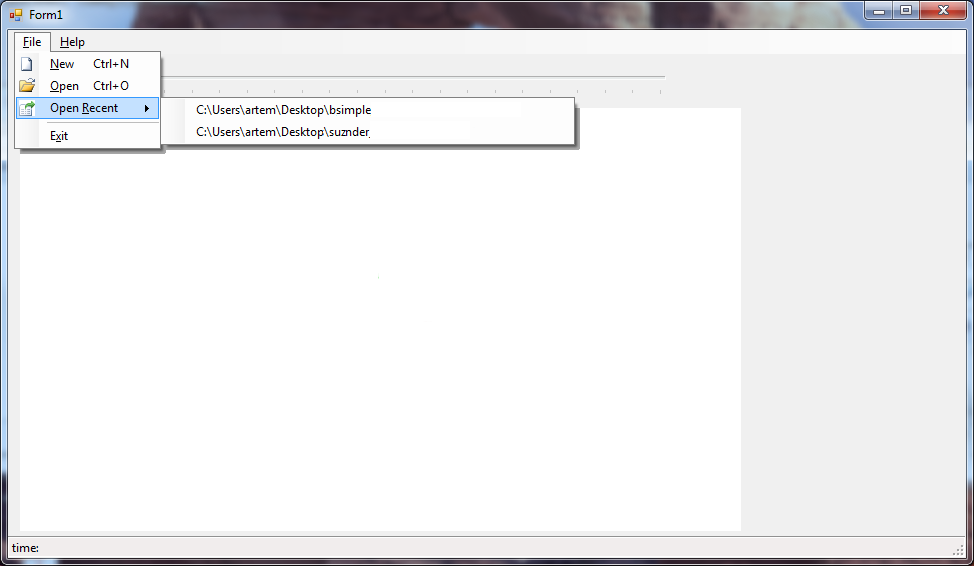
\includegraphics[width=0.8\textwidth]{../screenshots/file_menu_with_recent.png}
    \caption{Загрузка файла}
\end{figure}

Откроется диалог выбора файла:
\begin{figure}[h!]
    \centering
    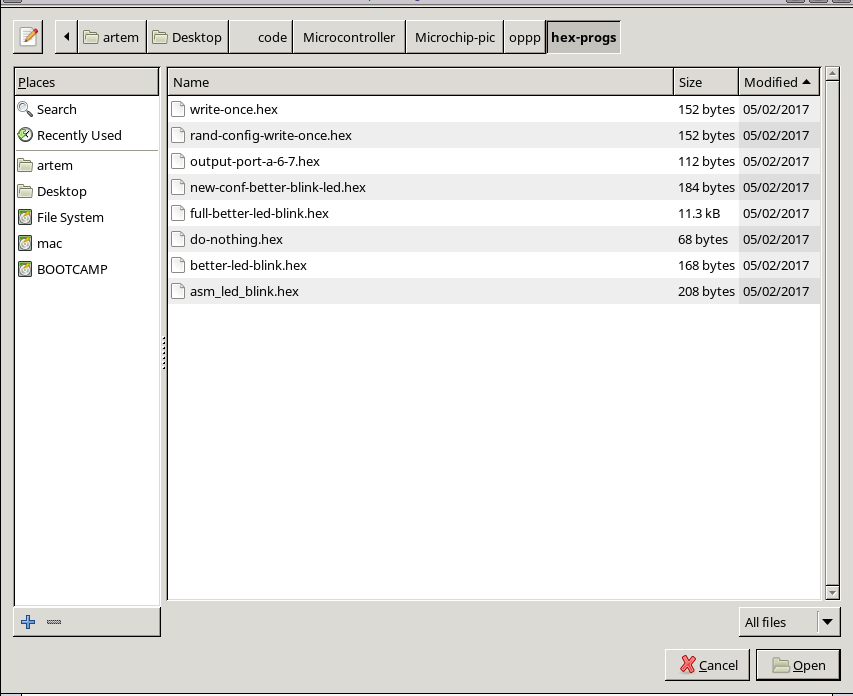
\includegraphics[width=0.5\textwidth]{../screenshots/open_file_dialog.png}
    \caption{Диалог выбора файла}
\end{figure}

После загрузки файла, его имя будет добавиленно в список недавно открытых файлов "Recent Files".

\subsection{Изменение положения камеры}
Изменять ракурс и приближение камеры можно при помощи мышки. Для приближения/отдаления используется колесо мышки. С помощью клавиш W,A,S,D можно двигать объект вверх, вправо, влево или вниз.

\subsection{Просмотр иерархии костей}
Структура загруженных данных отображена в виде дерева на панели справа. Выделенная на данный момент кость подсвеченна ярко-синим цветом.

\begin{figure}[h!]
    \centering
    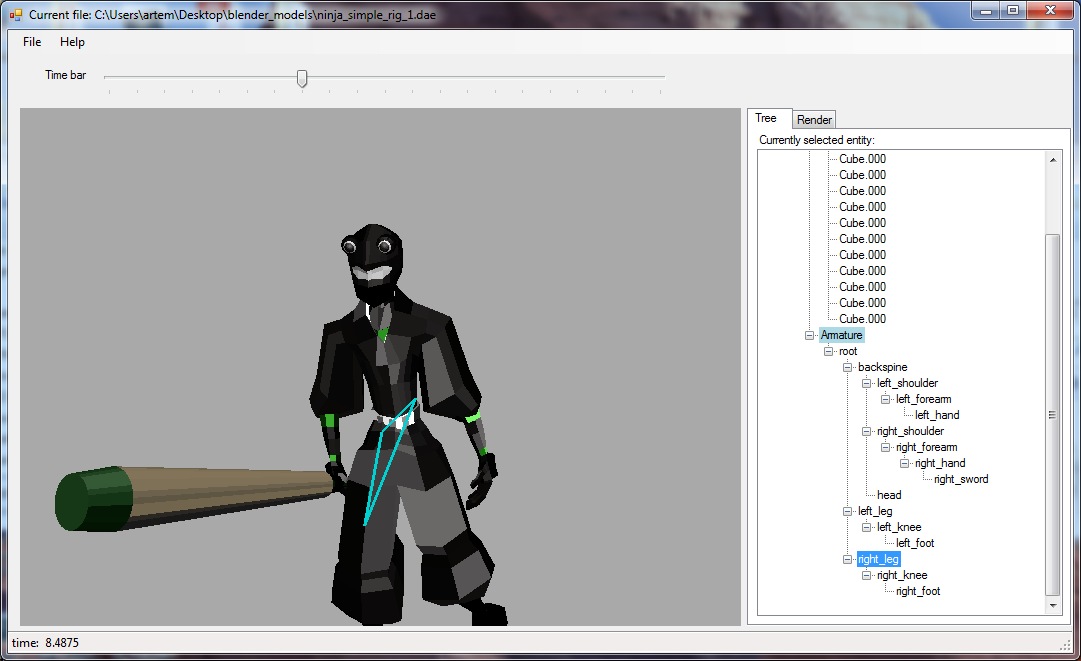
\includegraphics[width=0.8\textwidth]{../screenshots/frame_with_one_bone.png}
    \caption{Подсветка выбранной кости}
\end{figure}


\subsection{Изменение параметров отрисовки и анимации}
Элемент ScrollBar показывает текущий момент в анимации и предоставляет 
возможность перейти к любому моменту времени. 

\begin{figure}[h!]
    \centering
    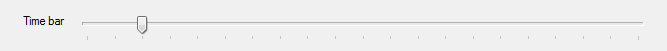
\includegraphics[width=0.5\textwidth]{../screenshots/time_bar.png}
    \caption{Элемент ScrollBar}
\end{figure}

Также есть панель для настоек работы программы позволяющая изменять следующие параметры:
\begin{my_enumerate}
\item Выбор между двумя видами камер в OpenGL, первый вид это камера движение которой сковано орбитой вокруг модели и другой тип это камера двигающаяся совершенно свободно.
\item Воспроизведение анимации.
\item Включение и выключение отрисовки с учетом нормалей.
\item Включение и выключение отрисовки с учетом характеристик материала.
\item Отрисовка всех костей скелета.
\end{my_enumerate}


\begin{figure}[h!]
    \centering
    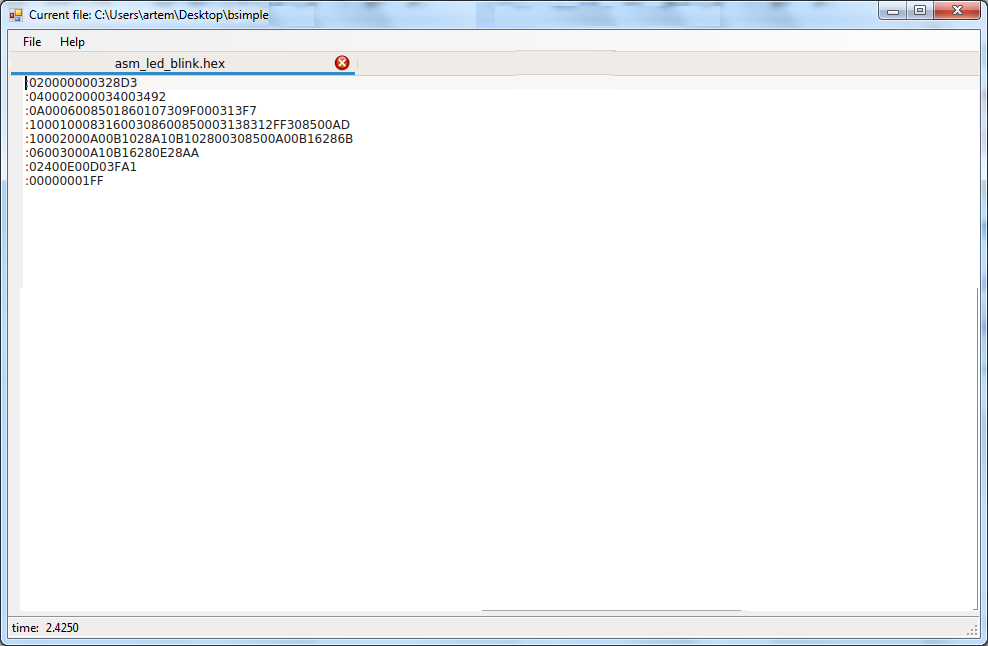
\includegraphics[width=0.8\textwidth]{../screenshots/interface_map.png}
    \caption{Справа: панель настойки отрисовки}
\end{figure}


\subsection{Всплывающие окна}
В случае если выбран файл не соответствующий требованиям входных данных отображается всплывающее окно:

\begin{figure}[h!]
    \centering
    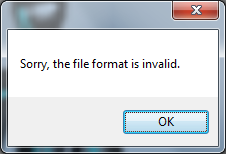
\includegraphics[width=0.3\textwidth]{../screenshots/error_message.png}
    \caption{Всплывающее окно}
\end{figure}


\subsection{Завершение работы с программой}
Происходит при нажатии на кнопку "Закрыть" в правом верхнем углу программы.
